\documentclass[ucs,9pt]{beamer}

% Copyright 2004 by Till Tantau <tantau@users.sourceforge.net>.
%
% In principle, this file can be redistributed and/or modified under
% the terms of the GNU Public License, version 2.
%
% However, this file is supposed to be a template to be modified
% for your own needs. For this reason, if you use this file as a
% template and not specifically distribute it as part of a another
% package/program, I grant the extra permission to freely copy and
% modify this file as you see fit and even to delete this copyright
% notice.
%
% Modified by Tobias G. Pfeiffer <tobias.pfeiffer@math.fu-berlin.de>
% to show usage of some features specific to the FU Berlin template.

% remove this line and the "ucs" option to the documentclass when your editor is not utf8-capable
\usepackage[utf8x]{inputenc}    % to make utf-8 input possible
\usepackage[english]{babel}     % hyphenation etc., alternatively use 'german' as parameter
\usepackage{attrib}

% Template for talks using the Corporate Design of the Freie Universitaet
%   Berlin, created following the guidelines on www.fu-berlin.de/cd by
%   Tobias G. Pfeiffer, <tobias.pfeiffer@math.fu-berlin.de>
% This file can be redistributed and/or modified in any way you like.
%   If you feel you have done significant improvements to this template,
%   please consider providing your modified version to
%   https://www.mi.fu-berlin.de/w/Mi/BeamerTemplateCorporateDesign

\usepackage{amsmath,dsfont,listings}

%%% FU logo
% small version for upper right corner of normal pages
\pgfdeclareimage[height=0.9cm]{university-logo}{FULogo_RGB}
\logo{\pgfuseimage{university-logo}}
% large version for upper right corner of title page
\pgfdeclareimage[height=1.085cm]{big-university-logo}{FULogo_RGB}
\newcommand{\titleimage}[1]{\pgfdeclareimage[height=2.92cm]{title-image}{#1}}
\titlegraphic{\pgfuseimage{title-image}}
%%% end FU logo

% NOTE: 1cm = 0.393 in = 28.346 pt;    1 pt = 1/72 in = 0.0352 cm
\setbeamersize{text margin right=3.5mm, text margin left=7.5mm}  % text margin

% colors to be used
\definecolor{text-grey}{rgb}{0.45, 0.45, 0.45} % grey text on white background
\definecolor{bg-grey}{rgb}{0.66, 0.65, 0.60} % grey background (for white text)
\definecolor{fu-blue}{RGB}{0, 51, 102} % blue text
\definecolor{fu-green}{RGB}{153, 204, 0} % green text
\definecolor{fu-red}{RGB}{204, 0, 0} % red text (used by \alert)

% switch off the sidebars
% TODO: loading \useoutertheme{sidebar} (which is maybe wanted) also inserts
%   a sidebar on title page (unwanted), also indents the page title (unwanted?),
%   and duplicates the navigation symbols (unwanted)
\setbeamersize{sidebar width left=0cm, sidebar width right=0mm}
\setbeamertemplate{sidebar right}{}
\setbeamertemplate{sidebar left}{}
%    XOR
% \useoutertheme{sidebar}

% frame title
% is truncated before logo and splits on two lines
% if neccessary (or manually using \\)
\setbeamertemplate{frametitle}{%
    \vskip-30pt \color{text-grey}\large%
    \begin{minipage}[b][23pt]{80.5mm}%
    \flushleft\insertframetitle%
    \end{minipage}%
}

%%% title page
% TODO: get rid of the navigation symbols on the title page.
%   actually, \frame[plain] *should* remove them...
\setbeamertemplate{title page}{
% upper right: FU logo
\vskip2pt\hfill\pgfuseimage{big-university-logo} \\
\vskip6pt\hskip3pt
% title image of the presentation
\begin{minipage}{11.6cm}
\hspace{-1mm}\inserttitlegraphic
\end{minipage}

% set the title and the author
\vskip14pt
\parbox[top][1.35cm][c]{11cm}{\color{text-grey}\inserttitle \\ \small \insertsubtitle}
\vskip11pt
\parbox[top][1.35cm][c]{11cm}{\small \insertauthor \\ \insertinstitute \\[3mm] \insertdate}
}
%%% end title page

%%% colors
\usecolortheme{lily}
\setbeamercolor*{normal text}{fg=black,bg=white}
\setbeamercolor*{alerted text}{fg=fu-red}
\setbeamercolor*{example text}{fg=fu-green}
\setbeamercolor*{structure}{fg=fu-blue}

\setbeamercolor*{block title}{fg=white,bg=black!50}
\setbeamercolor*{block title alerted}{fg=white,bg=black!50}
\setbeamercolor*{block title example}{fg=white,bg=black!50}

\setbeamercolor*{block body}{bg=black!10}
\setbeamercolor*{block body alerted}{bg=black!10}
\setbeamercolor*{block body example}{bg=black!10}

\setbeamercolor{bibliography entry author}{fg=fu-blue}
% TODO: this doesn't work at all:
\setbeamercolor{bibliography entry journal}{fg=text-grey}

\setbeamercolor{item}{fg=fu-blue}
\setbeamercolor{navigation symbols}{fg=text-grey,bg=bg-grey}
%%% end colors

%%% headline
\setbeamertemplate{headline}{
\vskip4pt\hfill\insertlogo\hspace{3.5mm} % logo on the right

\vskip6pt\color{fu-blue}\rule{\textwidth}{0.4pt} % horizontal line
}
%%% end headline

%%% footline
\newcommand{\footlinetext}{\insertshortinstitute, \insertshorttitle, \insertshortdate}
\setbeamertemplate{footline}{
\vskip5pt\color{fu-blue}\rule{\textwidth}{0.4pt}\\ % horizontal line
\vskip2pt
\makebox[123mm]{\hspace{7.5mm}
\color{fu-blue}\footlinetext
\hfill \raisebox{-1pt}{\usebeamertemplate***{navigation symbols}}
\hfill \insertframenumber}
\vskip4pt
}
%%% end footline

%%% settings for listings package
\lstset{extendedchars=true, showstringspaces=false, basicstyle=\footnotesize\sffamily, tabsize=2, breaklines=true, breakindent=10pt, frame=l, columns=fullflexible}
\lstset{language=Java} % this sets the syntax highlighting
\lstset{mathescape=true} % this switches on $...$ substitution in code
% enables UTF-8 in source code:
\lstset{literate={ä}{{\"a}}1 {ö}{{\"o}}1 {ü}{{\"u}}1 {Ä}{{\"A}}1 {Ö}{{\"O}}1 {Ü}{{\"U}}1 {ß}{\ss}1}
%%% end listings  % THIS is the line that includes the FU template!

\usepackage{arev,t1enc} % looks nicer than the standard sans-serif font
% if you experience problems, comment out the line above and change
% the documentclass option "9pt" to "10pt"

% image to be shown on the title page (without file extension, should be pdf or png)
\titleimage{vorratsdatenspeicherung}

\title[Seminar Datenschutz] % (optional, use only with long paper titles)
{Datenschutz}

\subtitle
{Vorratsdatenspeicherung}

\author[Manuel Polzhofer, Steve Dierker] % (optional, use only with lots of authors)
{M.~Polzhofer \and S.~Dierker}
% - Give the names in the same order as the appear in the paper.

\institute[FU Berlin] % (optional, but mostly needed)
{Freie Universität Berlin}
% - Keep it simple, no one is interested in your street address.

\subject{Seminar Datenschutz}
% This is only inserted into the PDF information catalog. Can be left
% out.

% you can redefine the text shown in the footline. use a combination of
% \insertshortauthor, \insertshortinstitute, \insertshorttitle, \insertshortdate, ...
\renewcommand{\footlinetext}{\insertshortinstitute, \insertshorttitle, \insertshortdate}

% Delete this, if you do not want the table of contents to pop up at
% the beginning of each subsection:
\AtBeginSubsection[]
{
  \begin{frame}<beamer>{Vorratsdatenspeicherung}
    \tableofcontents[currentsection,currentsubsection]
  \end{frame}
}

\begin{document}

\begin{frame}[plain]
  \titlepage
\end{frame}

\begin{frame}{Inhalt}
  \tableofcontents
  % You might wish to add the option [pausesections]
\end{frame}

%!TEX root = ../main.tex

\section{Einleitung}
  \begin{frame}
    \begin{itemize}
      \item \textbf{Vorratsdatenspeicherung}\\
        Unter einer Vorratsdatenspeicherung (VDS) versteht man die Speicherung personenbezogener Daten durch oder für öffentliche Stellen, ohne dass die Daten aktuell benötigt werden. Sie werden also nur für den Fall gespeichert, dass sie einmal benötigt werden sollten. In der rechtspolitischen Debatte bezieht sich der Begriff meist auf die Vorratsdatenspeicherung von Telekommunikations-Verbindungsdaten.
    \end{itemize}
  \end{frame}

%!TEX root = ../main.tex

\section{Geschichtliche Entwicklung}
  \subsection{Hintergrund}
    \begin{frame}
      \begin{itemize}
        \item
          Telekommunikation bedurfte früher die Verbindung von zwei Anschlüssen
        \item
          erste hälfte des 20. Jahrhunderts Einführung von Vermittlungsstellen
        \item
          Verbindungszähler addieren nur die Gebühren
        \item
          Einführung von Fangschaltungen
        \item 
         ab ca. 1980 Einführung von digitaler Vermittlungsgeräte
        \item
          Aufzeichnung von Rufnummern automatisch
        \item
          Erlaubte Speicherung nur zur Abrechnung

        % Kommentare
        % - Pruefung 2005 war ob und welche Dinge erlassen werden sollten
        % - Vorschlag von 2004 beinhaltete 36 Monate Speicherung, auch fuer Filesharing..
        % - Initiiert von Frankreich, Irland, Schweden und UK
        % - Ministerrat sieht es als seine Zustaendigkeit 'Dritte Saeule der EU'
        % - Parlament sieht es als seine 'Erste Saeule der EU'
        % - Kommision sagt beide

      \end{itemize}
    \end{frame}


%!TEX root = ../main.tex

\section{EU-Richtlinie}
    \subsection{2006/24/EG}
    \begin{frame}
      \frametitle{2006/24/EG}
      \begin{itemize}
        \item
          Richtlinie zur Vereinheitlichung der Vorratsspeicherung von Telekomunikationsdaten
        \item
          erster Entwurf August 2002 durch d"anische Ratspr"asidentschaft
        \item
          nach Madrider Anschl"agen vom 11. M"arz 2004 offizielle Beauftragung des Ministerrats mit Pr"ufung
        \item
          29. April 2004 erster Entwurf f"ur Rahmenbeschlu"s
        \item 
          7. Juli 2005 neuer Aufschwung durch Anschl"age in London
        \item
          21. September Vorlage durch EU-Kommission
        \item
          14. Dezember 2005, 378 zu 197 Stimmen im Europaparlament, somit die schellst verabschiedete Richtlinie der EU

        % Kommentare
        % - Pruefung 2005 war ob und welche Dinge erlassen werden sollten
        % - Vorschlag von 2004 beinhaltete 36 Monate Speicherung, auch fuer Filesharing..
        % - Initiiert von Frankreich, Irland, Schweden und UK
        % - Ministerrat sieht es als seine Zustaendigkeit 'Dritte Saeule der EU'
        % - Parlament sieht es als seine 'Erste Saeule der EU'
        % - Kommision sagt beide

      \end{itemize}
    \end{frame}

    \begin{frame}
      \frametitle{2006/24/EG}
      \begin{itemize}
        \item 
          Mitgliedsstaaten haben bis zum 15. September 2007 Zeit zur Umsetzung
        \item 
          E-Mail, Internet und VoIP sind bis 15. M"arz 2009 umzusetzen
        \item
          erste Klage von Irland am 6. Juli 2006, Rechtsgrundlage mit Binnenmarktkompetenz (Artikel 95 EG) nicht ausreichend
        \item
          30. Mai 2006 Urteil zu "ubermittlung von Fluggastdaten.\\
          'EG-Rechtsakte zum Schutz der öffentlichen Sicherheit und zu Strafverfolgungszwecken sind unzulässig'
        \item 
          8. April 2014 erkl"art der Europ"aische Gerichtshof die Richtlinie f"ur Ung"ultig, versto"st gegen die Charta der Grundrechte der Europ"aischen Union
      \end{itemize}
    \end{frame}

    \begin{frame}
      \frametitle{R"uchverfolgng und Identifizierung der Quelle/des Empf"angers}
      \begin{itemize}
        \item Telefonnetz
        \begin{itemize}
          \item Art des Vorgangs
          \item Rufnummer des Anschlusses
          \item Name und Anschrift des Teilnehmers
        \end{itemize}
        \item Internet
        \begin{itemize}
          \item Art des Vorgangs
          \item Benutzerkennung
          \item Name und Anschrift des Teilnehmers
        \end{itemize}
      \end{itemize}
    \end{frame}

    \begin{frame}
      \frametitle{Bestimmung von Datum, Uhrzeit, Dauer einer Kommunikation}
      \begin{itemize}
        \item Telefonnetz
        \begin{itemize}
          \item Datum und Uhrzeit zu Beginn und Ende des Vorgangs
        \end{itemize}
        \item Internet
        \begin{itemize}
          \item Datum und Uhrzeit der An- und Abmeldung
          \item zugeh"orige IP-Adresse
          \item Benutzerkennung des Nutzers
          \item Datum und Uhrzeit der An- und Abmeldung bei E-Mail/VoIP-Diensten
        \end{itemize}
      \end{itemize}
    \end{frame}

    \begin{frame}
      \frametitle{Bestimmung der Endeinrichtung}
      \begin{itemize}
        \item Telefonnetz
        \begin{itemize}
          \item internationale Mobilteilnehmerkennung (IMSI)
          \item internationale Mobilfunkger"atekennung (IMEI)
          \item bei annonymen Diensten Datum, Uhrzeit und Cell-ID der Aktivierung
        \end{itemize}
      \end{itemize}
    \end{frame}

    \begin{frame}
      \frametitle{Standortbestimmung mobiler Endger"ate}
      \begin{itemize}
        \item Cell-ID bei Beginn der Verbindung
        \item Daten zur geographischen Ortung von Funkzellen w"ahrend der Kommunikation
      \end{itemize}
    \end{frame}
%!TEX root = ../main.tex

\section{Umsetzung in Deutschland}

  \begin{frame}
  \frametitle{Gesetz zur Neuregelung der Telekommunikationsüberwachung}
    \begin{itemize}
      \item 
        regelte vom 1. Januar 2008 bis 2. M"arz 2010 die Vorratsdatenspeicherung
      \item 
        entgegen der EU-Richtlinie waren ab 1. Januar 2009 auch nicht kommerzielle Dienste zur Speicherung verpflichtet
      \item 
        Vorratsdatenspeicherung bei nicht Verpflichtung bestraft mit Geldbu"se bis 10000 Euro (siehe \S 149 Abs. 1 Nr 17 TKG)
    \end{itemize}
  \end{frame}

  \begin{frame}
    \frametitle{Nutzung der Daten}
    \begin{itemize}
      \item Verfolgung von Straftaten
      \item Abwehr von erheblichen Gefahren f"ur die "offentliche Sicherheit
      \item Erf"ullung der Aufgaben von Verfassungsschutzbeh"orden, Bundesnachrichtendiensten und Milit"arischen Abschirmdienstes
      \item Asuk"unfte "uber Identit"at von Telekomunikatons- und Internetnutzern nach \S 113
      \item Urheberrechtsverletzungen im Internet
    \end{itemize}
  \end{frame}

  \begin{frame}
    \frametitle{Verfassungsbeschwerde}
    \begin{itemize}
      \item 31. Dezember 2007 wurde vom Arbeitskreis Vorratsdatenspeicherung initiierte Sammel-Verfassungsbeschwerde eingereicht
      \item insgesamt 34939 Beschwerdef"uhrer
      \item 11. M"arz 2008 einstweilige Verf"ugung, Nutzung der Daten nur noch bei schweren Straftaten
      \item Bundesregierung zu Bericht bis 1. September "uber praktische Ausirkungen verpflichtet
    \end{itemize}
  \end{frame}

  \begin{frame}
    \frametitle{Urteil}
    \begin{itemize}
      \item Vorschriften zur Vorratsdatenspeicherung sind verfassungswidrig
      \item Gesetz in seiner Form verst"o"st gegen Art. 10 Abs. 1 GG
      \item nicht generell Unvereinbar mit Gesetz
      \item Daten sollten dezentral gespeichert und besonders gesichert werden
      \item Beh"orden nur bei genau spezifizierten F"allen zugriff gew"ahren
      \item Ermittlung der IP-Adresse selbst bei Ordungswidrigkeiten zul"assig
    \end{itemize}
  \end{frame}

%!TEX root = ../main.tex

\section{Technische Details}
    \begin{frame}
      \frametitle{Kosten}
      \begin{itemize}
        \item 
          Kosten laut Verband der deutschen Internetwirtschaft, 205 Millionen Euro Investition, min. 50 Millionen pro Jahr, Appendix \cite{kostenVDS}
        \item
          Private E-Mail Provider sowie Anonyme E-Mail Provider nicht betroffen
        \item 
          Provider bis '1000  Teilnehmern' ausgeschlossen, Appendix \cite{emailAusnahme}
      \end{itemize}
    \end{frame}

  \begin{frame}
    \frametitle{Technik IPv4}
    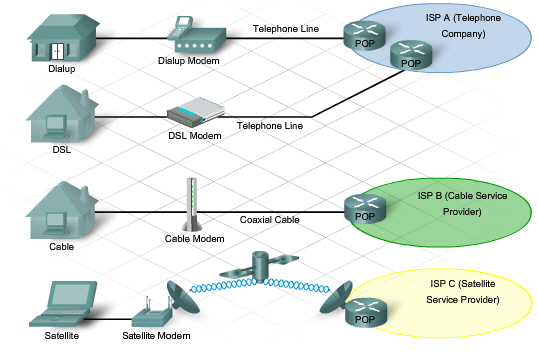
\includegraphics[scale=0.65 ]{sections/img/internet_ipv4.jpg}
  \end{frame}

  \begin{frame}
    \frametitle{Technik IPv6}
    \begin{itemize}
      \item Speicherung der dynamischen Mappings von IPv4 Adressen obsolet
      \item Moeglichkeit jedem Ger"at eine statische Adresse zu zuordnen
      \item \( 16.777.216 \) Adressen in IPv4 \( /24 \), entspricht \( /104 \) in IPv6
      \item IPv6 {\em Privacy Extension} f"ugt Zufall in die Adressen ein zur Verhinderung statischer Adressen f"ur ein Ger"at, Appendix \cite{RFC4941}
    \end{itemize}
  \end{frame}
%!TEX root = ../main.tex
\section{Kritik}
  \subsection*{Unverhältnismäßige geringer Nutzen}
    \begin{frame}<beamer>{Unverhältnismäßige geringe Nutzung}
      \begin{itemize}
        \item
          Abschreckungfaktor ist nicht vorhanden.
        \item
         Umgehungsmöglichkeiten sind auch für Laien möglich.
        \begin{itemize}
          \item TOR-Netzwerk
          \item alternative Emaildienste
          \item bei SMS auf Alternativen umsteigen (zb. Whatsapp)
        \end{itemize}
        \item Durch Vorratsdatenspeicherung hätte weder 9/11 als auch die Attentate in Großbritannien 2005 verhindert werden können
      \end{itemize}
    \end{frame}

\begin{frame}<beamer>{Schwere Strafdaten in Deutschland Statstik}
\begin{itemize}
        \item Schwere Strafdaten in Deutschland Statstik
        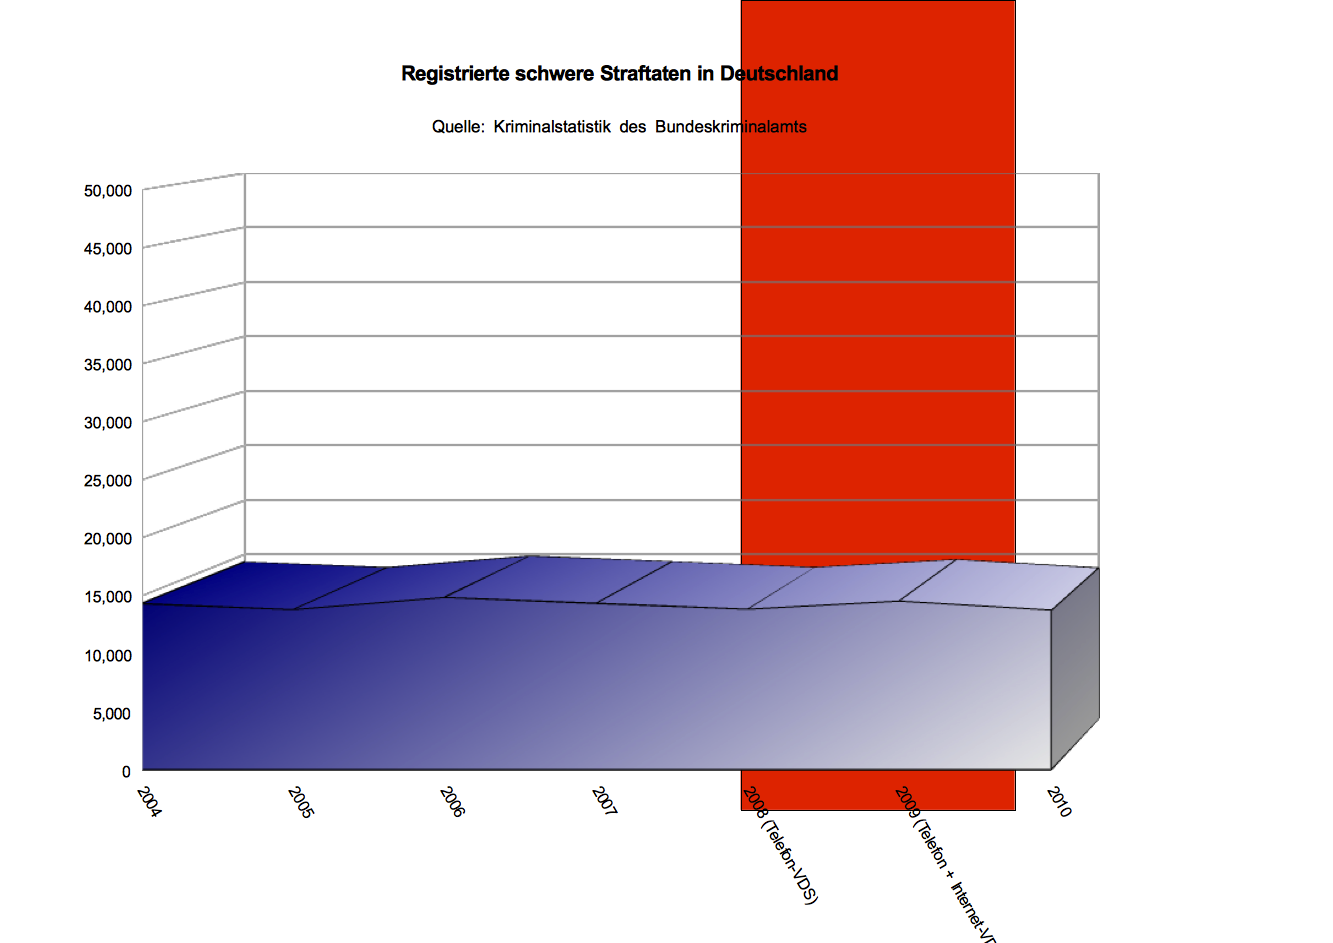
\includegraphics[height=1\textheight]{sections/img/schwere_verbrechen_in_DE.png}
    \end{itemize}
    \end{frame}
    
    \begin{frame}<beamer>{Schwere Verbrechen in Deutschland Aufklärung Statistik}
\begin{itemize}
        \item Schwere Verbrechen in Deutschland Aufklärung Statistik
        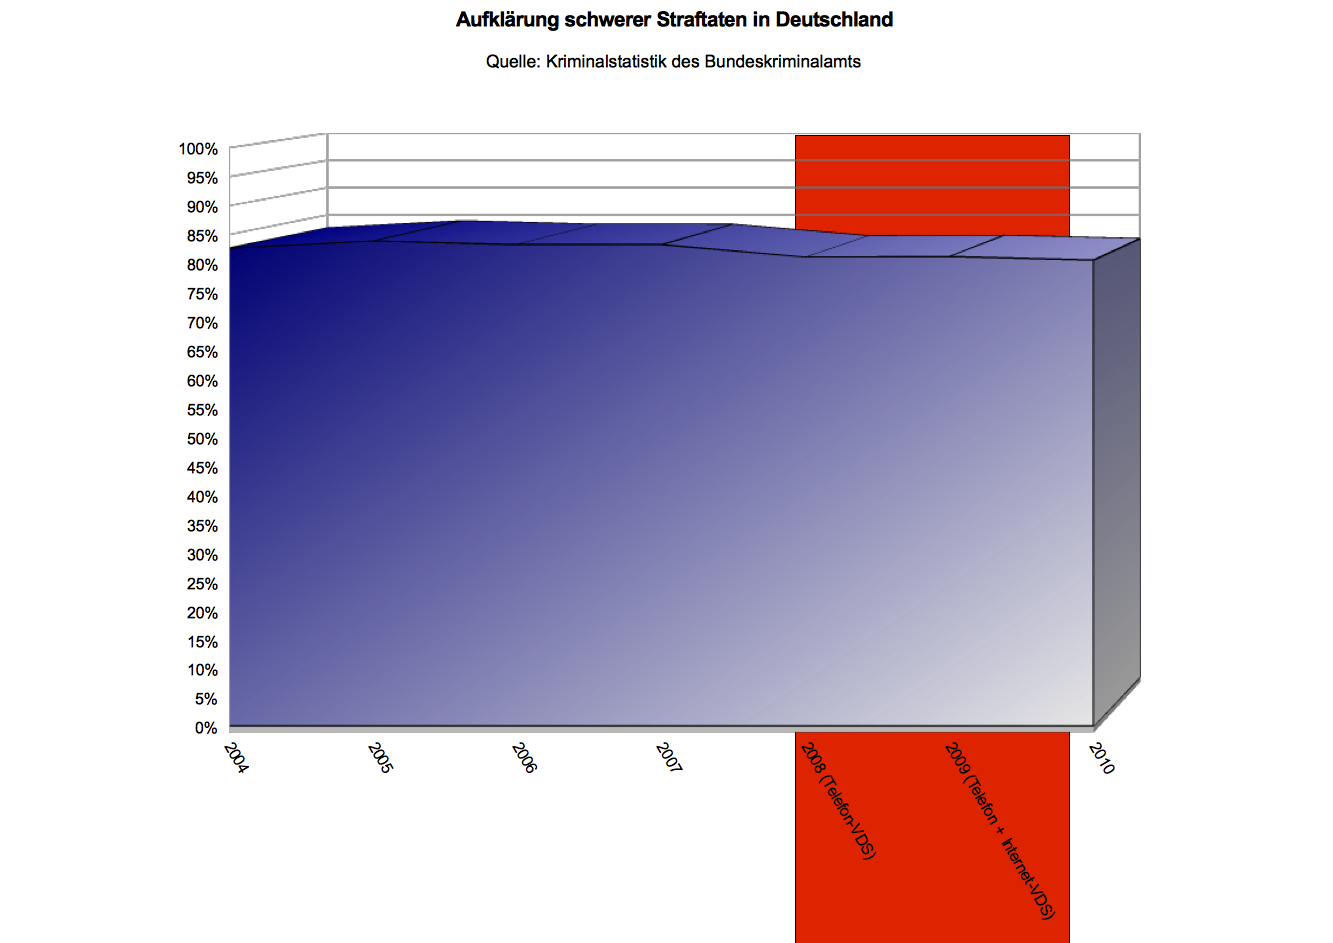
\includegraphics[height=1\textheight]{sections/img/aufklaerung_in_DE.png}
    \end{itemize}
    \end{frame}
      \begin{frame}<beamer>{Internetstrafdaten in Deutschland Statistik}
\begin{itemize}
        \item Internetstrafdaten in Deutschland Statistik
        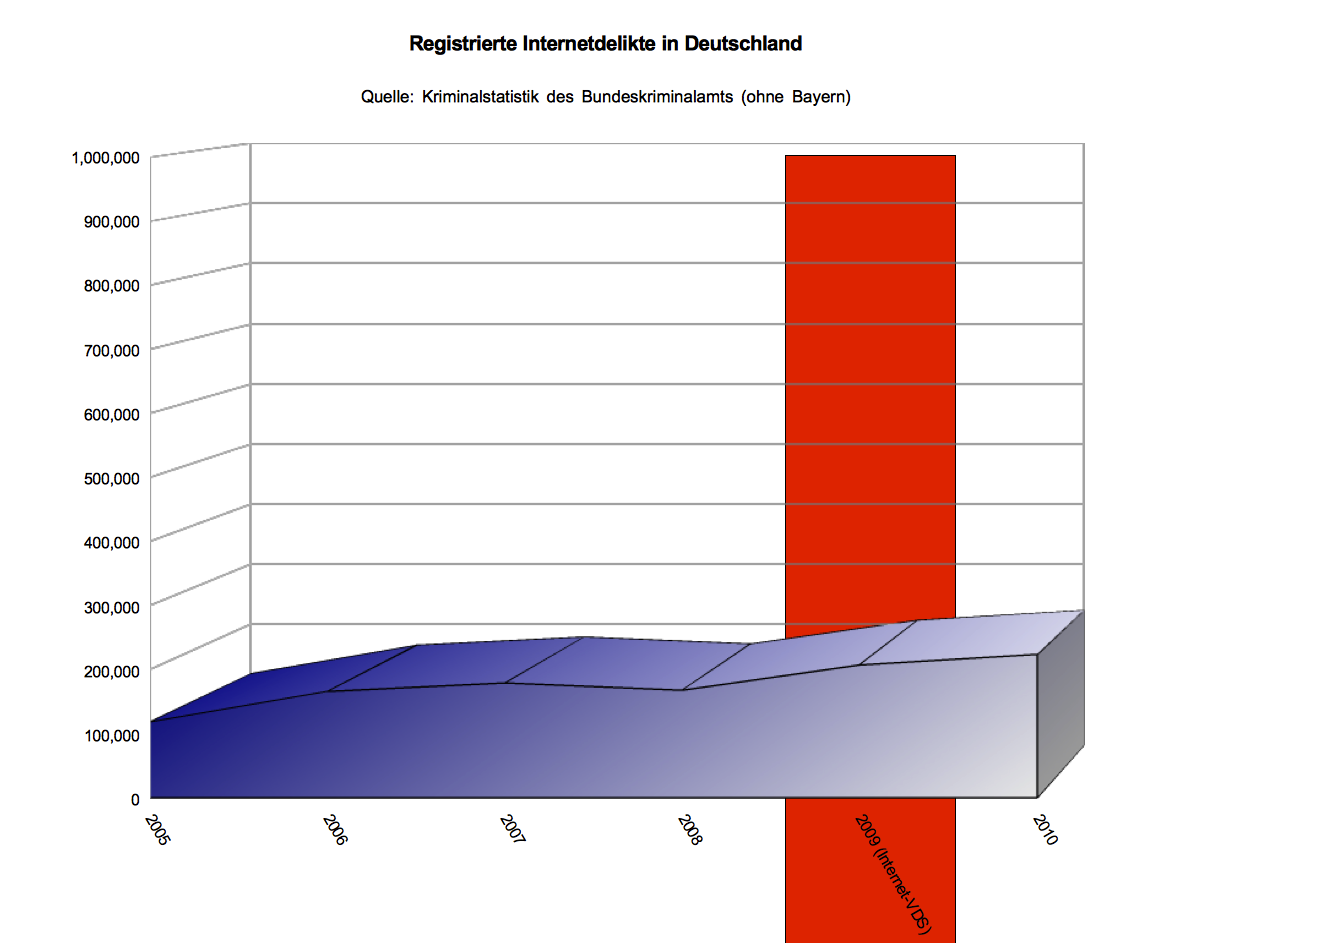
\includegraphics[height=1\textheight]{sections/img/internet_delikte_in_DE.png}
    \end{itemize}
    \end{frame}
          \begin{frame}<beamer>{Internetstrafdaten in Deutschland Aufklärung Statistik}
\begin{itemize}
        \item Internetstrafdaten in Deutschland Aufklärung Statistik
        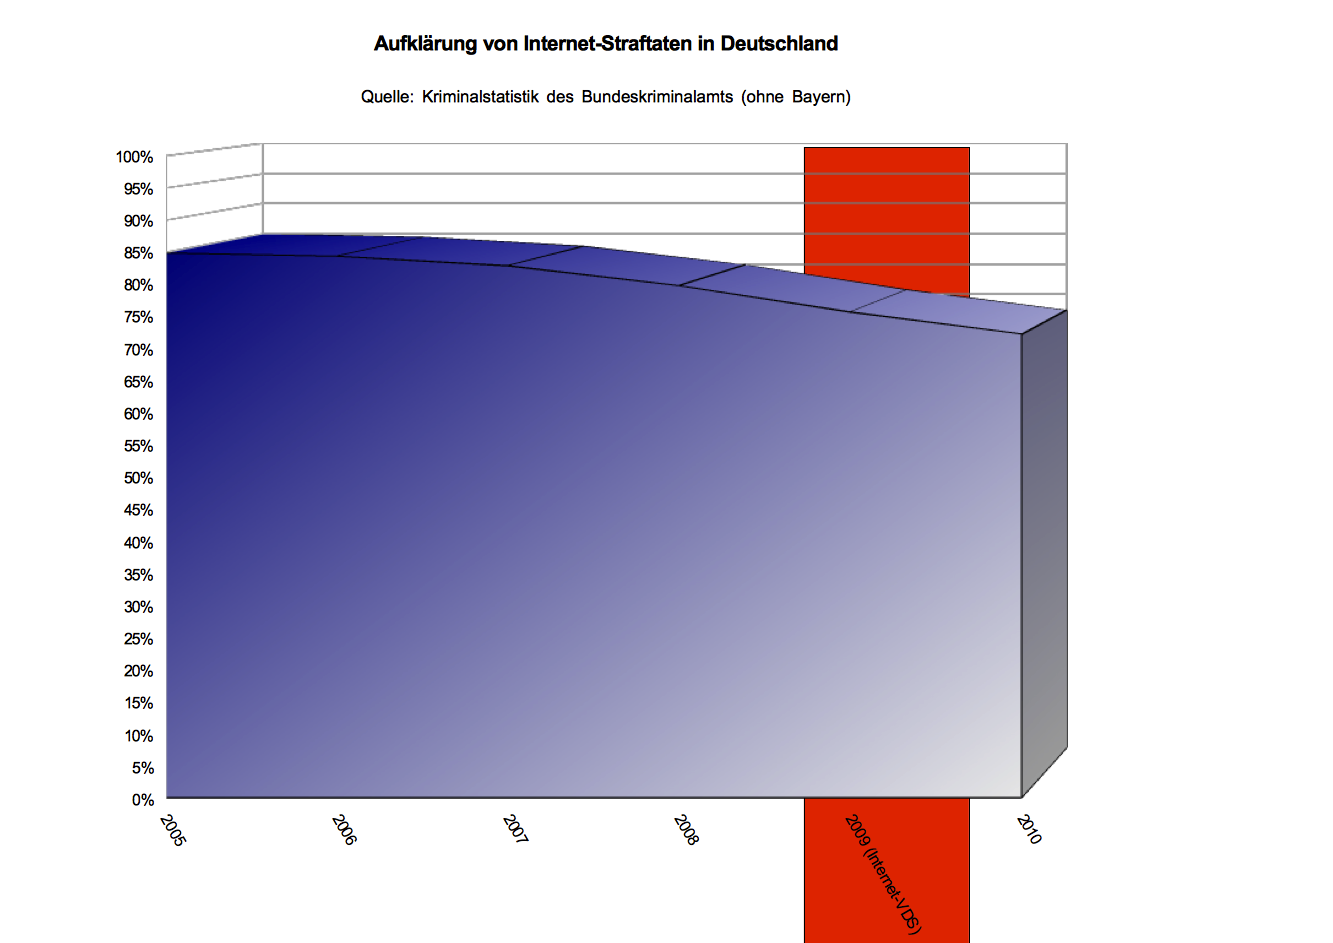
\includegraphics[height=1\textheight]{sections/img/aufklaerung_internetdelikte_DE.png}
    \end{itemize}
    \end{frame}
              \begin{frame}<beamer>{Aufklärungsquote Allgmein}
        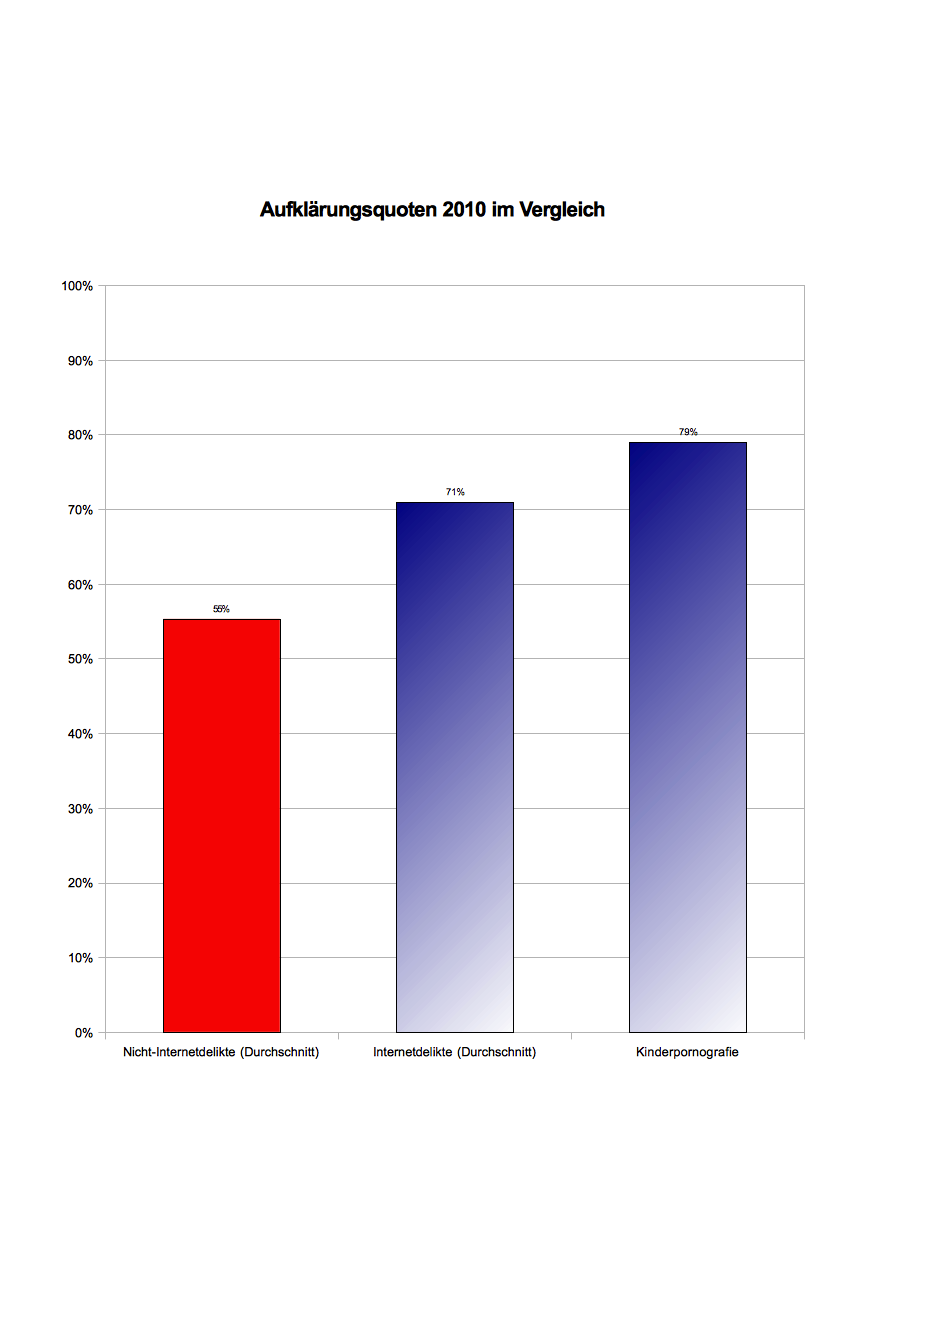
\includegraphics[height=1.25\textheight]{sections/img/aufklaerung.png}
      \end{frame}
              \begin{frame}<beamer>{Interpretation der Statistik des Bundeskriminalamtes}
\begin{itemize}
        \item Die VDS brachte keine Erhöhte Aufklärungsquote
        \item Es konnte keine Senkung der Kriminalitätsrate festgestellt werden
        \item Die Aufklärungsrate der Internetstraftaten sank im Zeitraum der VDS
    \end{itemize}
    \end{frame}
       \begin{frame}<beamer>{Bilanz der Vorratsdatenspeicherung in Österreich}
        \begin{itemize}
        \item 312 Fälle gab es Auskunft über Vorratsdatenspeicherung
        \item 438 Delikte wurde Vorratsdatenspeicherung abgefragt
        \item 161 erledigten Rechtssachen soll in 71 Fällen die Vorratsdatenspeicherung eine Betrag zur Aufklärung geleistet haben
        \item die meisten Abfragen gab es nicht bei schweren Verbrechen, wie Terrorismus und Mord sondern
        \item die meisten gab es bei Diebstahl(106) und Stalking
        \item Kosten für die Steuerzahler bisher 2,3 Millionen Euro
        \item Man rechnet mit jährliche Gesamtkosten von 8 Millionen Euro.
        \item Stand: 09.07.2013 
         \end{itemize}
    \end{frame}
    \begin{frame}<beamer>{Straftaten in Osterreich Vergleich}
      \begin{quote}
        Dennoch zeigten die Daten der österreichischen Vorratsdatenspeicherung, daß die angeblich schwersten Straftaten, bei denen die Datensätze abgerufen werden sollten, in Wahrheit in erster Linie Diebstahlsdelikte waren, außerdem Stalking. Bei Organisierter Kriminalität oder Taten, die als Terror definiert sind, wurden die zwangsweise gespeicherten Daten in genau null Fällen verwendet.

        \attrib{Chaos Computer Club}
      \end{quote}
    \end{frame}



  \subsection*{Missbrauch und Irrtumsrisiko}
    \begin{frame}<beamer>{Missbrauch und Irrtumsrisiko}
      \begin{itemize}
        \item
          Telekommunikationsdaten haben eine sehr hohe Aussagekraft
      \begin{itemize}
         \item mit Methoden von Data-mining können scheinbar belanglose Daten eine hohe Aussagekraft bekommen
      \end{itemize}
        \item
          Rückschlüsse auf die gesamte Lebensituation möglich
 \item viele Interessensgruppen haben Interesse an den sensiblen Daten
          \begin{itemize}
         \item Behörden/Staat
         \item politische Gruppierungen
         \item Personen aus Privatenumfeld
      \end{itemize}
 
      \end{itemize}
    \end{frame}

  \subsection*{Juristische Argumente}
    \begin{frame}<beamer>{Juristische Argumente}
      \textbf{Verstoß gegen Europarecht}
      \begin{quote}
        Der Gerichtshof sieht in der Verpflichtung zur Vorratsspeicherung dieser Daten und der Gestattung des Zugangs der zuständigen nationalen Behörden zu ihnen einen besonders schwerwiegenden Eingriff der Richtlinie in die Grundrechte auf Achtung des Privatlebens und auf Schutz personenbezogener Daten.

        \attrib{Gerichtshof der Europäischen Union}
      \end{quote}
    \end{frame}

    \begin{frame}<beamer>{Juristische Argumente}
      \textbf{Verstoß gegen Europarecht}
      \begin{quote}
        Zwar ist die nach der Richtlinie vorgeschriebene Vorratsspeicherung der Daten zur Erreichung des mit ihr verfolgten Ziels geeignet, doch beinhaltet sie einen Eingriff von großem Ausmaß und von besonderer Schwere in die fraglichen Grundrechte, ohne dass sie Bestimmungen enthielte, die zu gewährleisten vermögen, dass sich der Eingriff tatsächlich auf das absolut Notwendige beschränkt.

        \attrib{Gerichtshof der Europäischen Union}
      \end{quote}
    \end{frame}

    \begin{frame}<beamer>{Juristische Argumente}
      \textbf{Verstoß gegen deutsches Recht}
      \begin{quote}
        Eine sechsmonatige, vorsorglich anlasslose Speicherung von Telekommunikationsverkehrsdaten durch private Diensteanbieter, wie sie die Richtlinie 2006/24/EG des Europäischen Parlaments und des Rates vom 15. März 2006 (ABl L 105 vom 13. April 2006, S. 54; im Folgenden: Richtlinie 2006/24/EG) vorsieht, ist mit Art. 10 GG nicht schlechthin unvereinbar; auf einen etwaigen Vorrang dieser Richtlinie kommt es daher nicht an.

        \attrib{Bundesverfassungsgericht}
      \end{quote}
    \end{frame}

    \begin{frame}<beamer>{Juristische Argumente}
      \textbf{Versto"s gegen die Europ"aische Menschenrechtskonvention}
      \begin{quote}
        Die Erfassung aller Verbindungsdaten könne 'nicht als vereinbar mit den Bestimmungen der Verfassung und der Europäischen Menschenrechtskonvention erachtet werden'.

        \attrib{"Ubersetzung durch AK-Vorratsdatenspeicherung}
      \end{quote}
    \end{frame}

    \subsection*{Demonstrationen}
    \begin{frame}<beamer>{Protestbewegungen}
      \begin{figure}
        \begin{subfigure}[b]{0.5\textwidth}
          \begin{itemize}
            \item Arbeitskreis Vorratsdatenspeicherung
            \item Unterst"utzung aus unterschiedlichsten Bereichen z.B.:
              \begin{itemize}
                \item CCC
                \item Deutsche Journalistinnen- und Journalisten-Union
                \item Internationale Liga für Menschenrechte
                \item Deutscher Anwaltverein
              \end{itemize}
            \item 11. Oktober 2008: Demonstration {\em Freiheit statt Angst} mit 15.000 Teilnehmern in Berlin
          \end{itemize}
        \end{subfigure}
        \begin{subfigure}[b]{0.3\textwidth}
          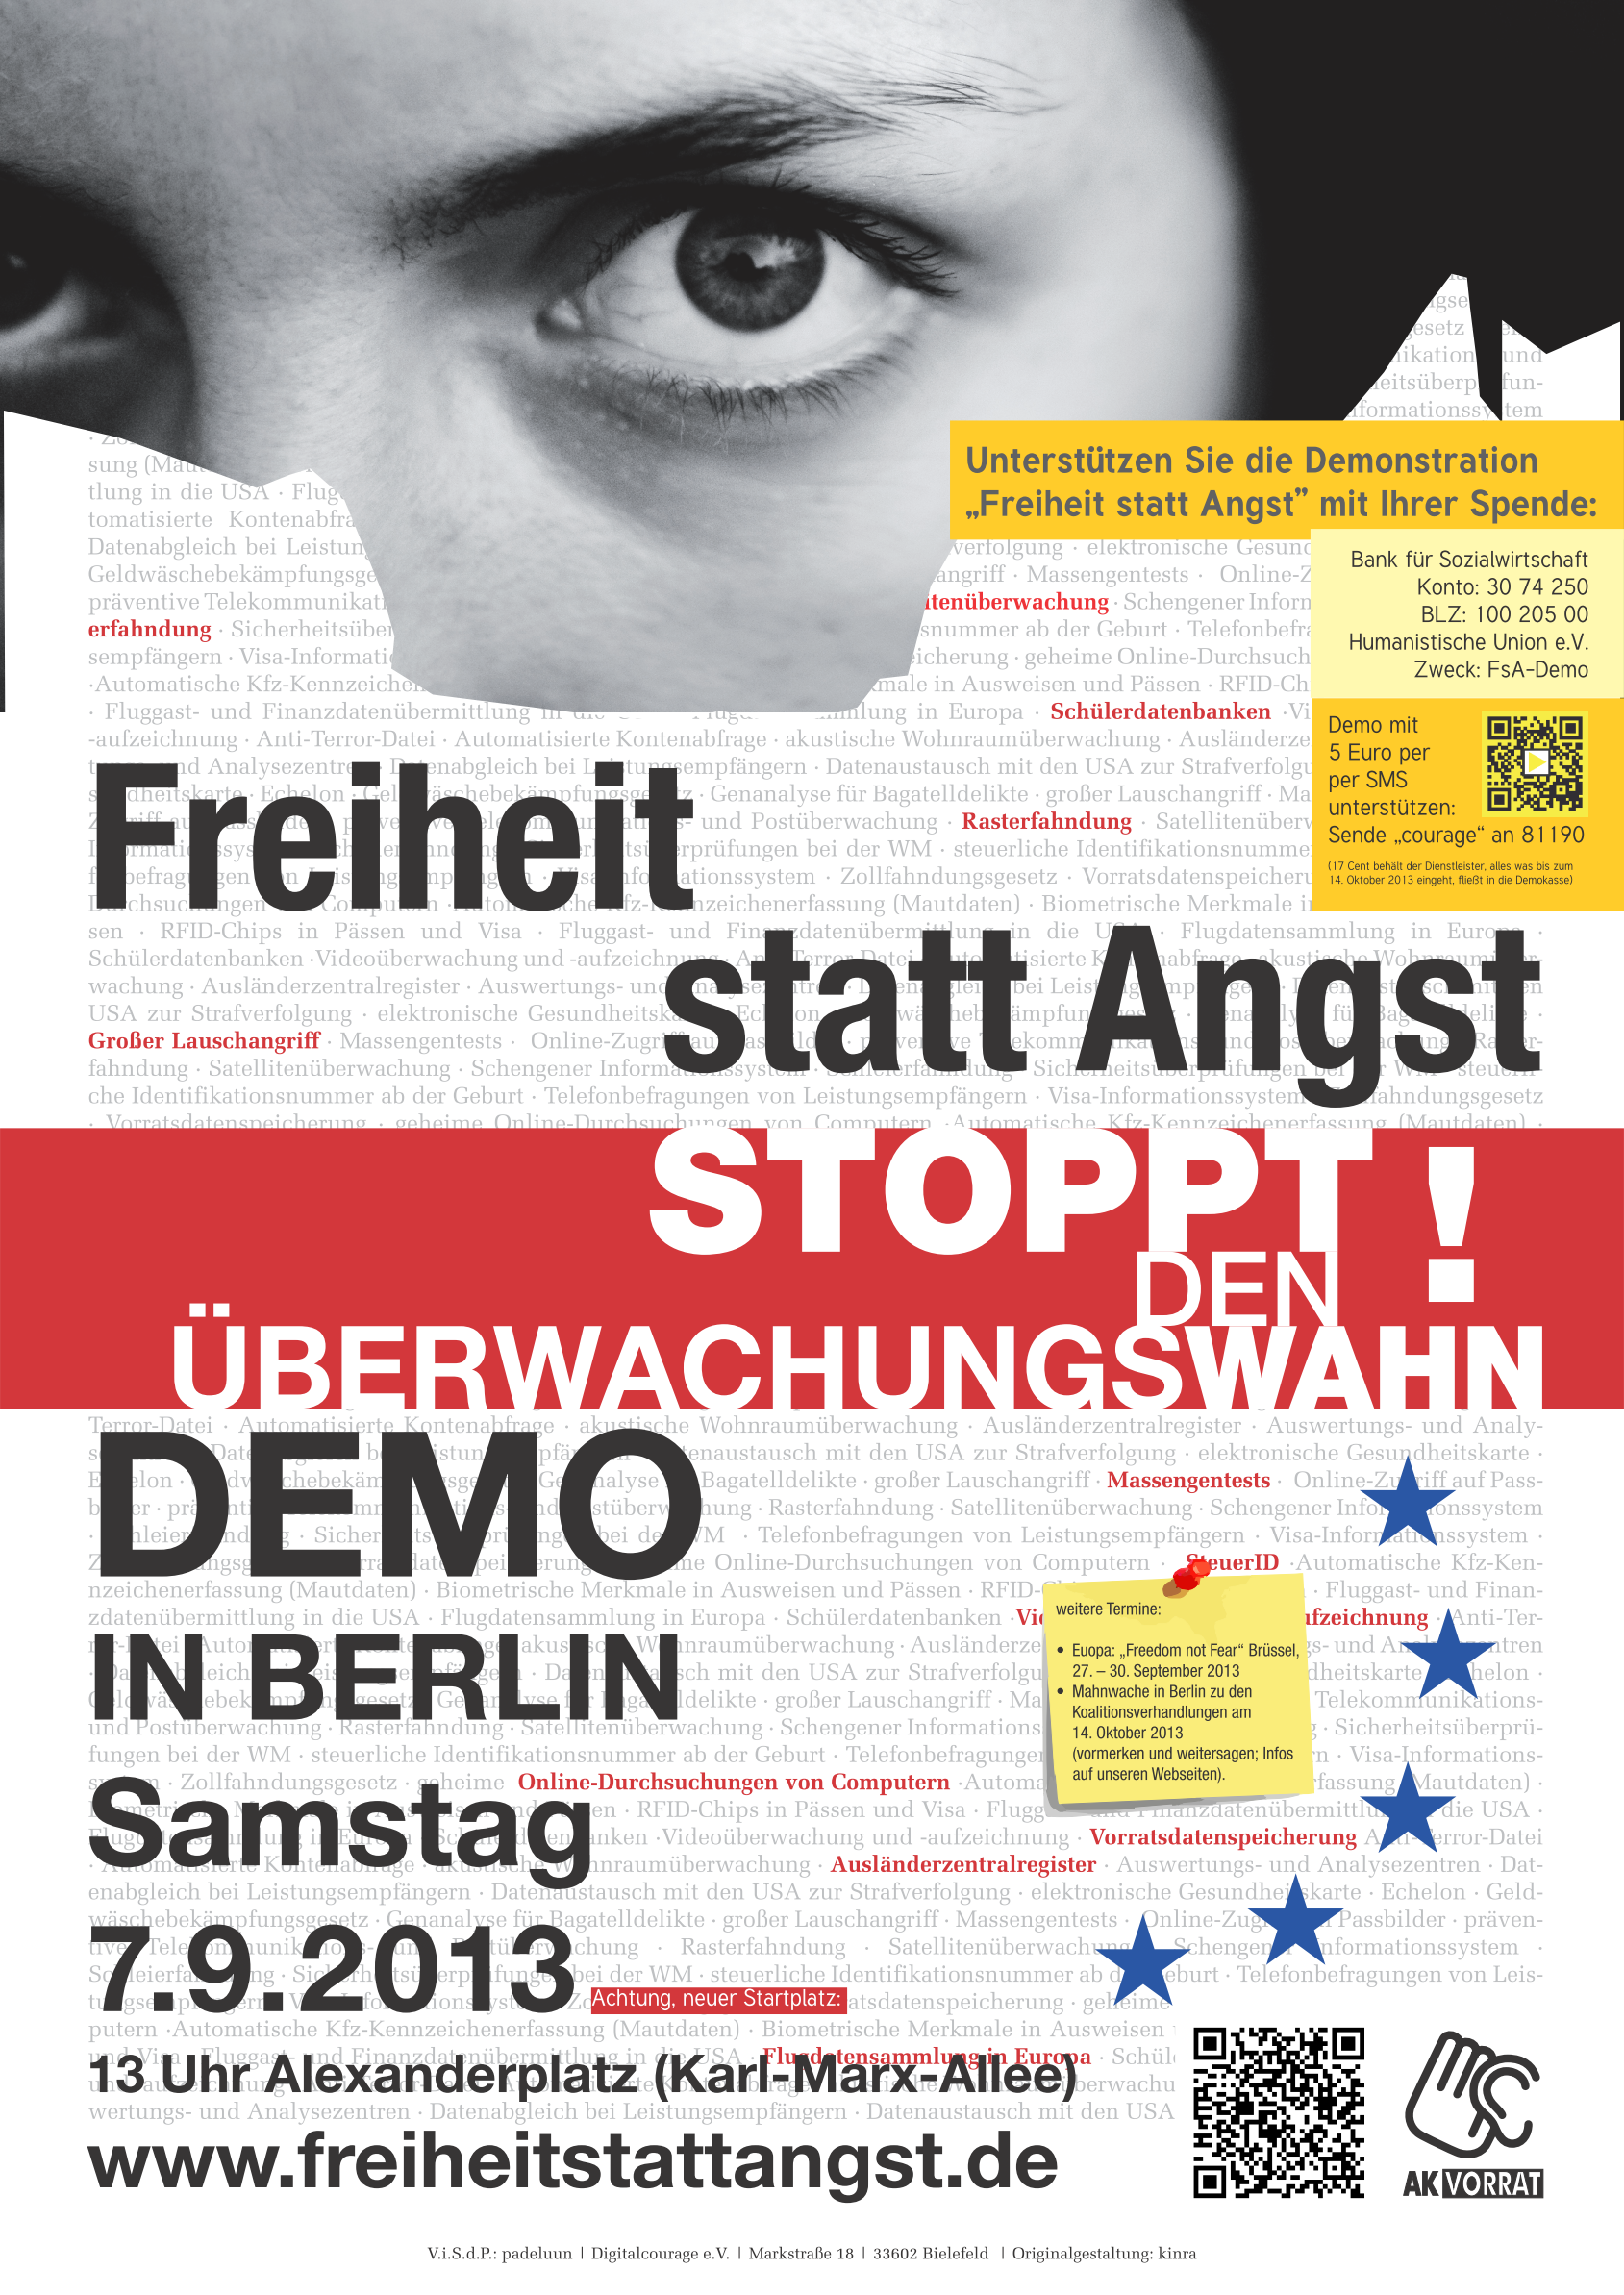
\includegraphics[scale=0.05]{sections/img/freiheit_statt_angst.png}
          \caption{Freiheit statt Angst}
          \label{fig:tiger}
        \end{subfigure}
      \end{figure}
    \end{frame}
    \begin{frame}<beamer>{Meinungsumfrage zur Vorratsdatenspeicherung}
       \begin{itemize}
        \item Nach einer Umfrage des Meinungsinstitutes Allenbach im Jahr 2011
        \item 66 Prozent der Deutschen befürworteten eine Begrenzung auf Strafverdachtsfälle
        \item 19 Prozent sprachen sich für die anlasslose VDS aus
        \item 15 Prozent zeigten sich unentschieden oder verweigerten eine Antwort
      \end{itemize}
    \end{frame}

    \begin{frame}<beamer>{Kritik aus dem historischen Kontext}
      \begin{figure}
        \begin{subfigure}[b]{0.5\textwidth}
          \begin{itemize}
            \item totalitäre Überwachung im 3. Reich durch Gestapo
            \item Überwachung der Stasi in der DDR 
            \item Befürchtung die Ausweitung der Überwachung könnte die Demokratie aushöhlen und letztlich abschaffen.
          \end{itemize}
        \end{subfigure}
        \begin{subfigure}[b]{0.3\textwidth}
          
\includegraphics[scale=0.2]{sections/img/stasi.png}
          \caption{Stasi 2.0}
          \label{fig:stasi}
        \end{subfigure}
      \end{figure}
    \end{frame}

%!TEX root = ../main.tex
\section{Umgehungsmöglichkeiten}
  \subsection{Ausweichen zu Alternativen}
    \begin{frame}
      \begin{itemize}
        \item Briefverkehr
        \item Apps für SMS versandt. (Whatsapp)
        \item alternative Emailprovider welche nicht überwacht werden
        

      \end{itemize}
    \end{frame}
      \subsection{VPN,Proxy,TOR}
    \begin{frame}
      \begin{itemize}
        \item VPN - Virtual Private Network 
        \item Webproxy
               \begin{itemize}
         \item Computer verbindet sich über das Internet zu einem Server und surft über diesem weiter
         \item Die Vorratsdatenspeicherung würde nur die Adresse des Webproxys speichern.
  
      \end{itemize}
      \end{itemize}
    \end{frame}
        \begin{frame}
      \begin{itemize}
        \item TOR
        \item TOR ist ein Netzwerk zu Anonymisierung von Verbindungsdaten
        \item Verwendung für Webbrowsing, Instance Messaging IRC,SSH,Email
        \item TOR basiert auf dem Prinzip des Onion-Routings
   
      \end{itemize}
    \end{frame}







%!TEX root = ../main.tex
\section{Politische Debatte}
  \subsection{Standpunkte einzelner Parteien}
        \begin{frame}<beamer>{Abstimmungsverhalten im Deutschen Bundestag}
\begin{itemize}
        \item Abstimmungsverhalten bei der Einführung der VDS
        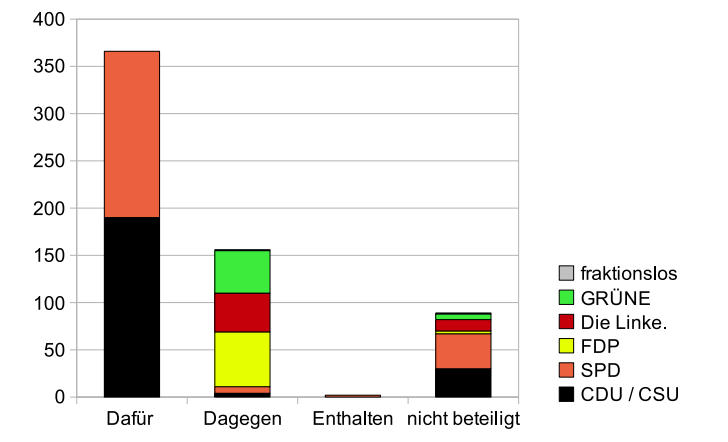
\includegraphics[height=0.9\textheight]{sections/img/abstimmung.png}
    \end{itemize}
    \end{frame}
  
  
    \begin{frame}<beamer>{Standpunkte der CDU}
       \begin{itemize}
        \item setzte sich von Anfang an für VDS ein
        \begin{itemize}
        \item Argumentation: zunehmende Bedrohung durch Terror, Kinderpornographie
         \end{itemize}
        \item 23. April 2014: Das Urteil des Europäischen Gerichtshofs "verdammt uns keineswegs zur Untätigkeit", sagte CDU-Vize Thomas Strobl der "Stuttgarter Zeitung" 
  
      \end{itemize}
    \end{frame}

  \begin{frame}<beamer>{Standpunkte der SPD}
        \begin{quote}
Trotz schwerwiegender politischer und verfassungsrechtlicher
Bedenken werden wir im Ergebnis dem Gesetzentwurf aus
folgenden Erwaegungen zustimmen. Erstens. Grunds¨atzlich
stimmen wir mit dem Ansatz der Bundesregierung und der
Mehrheit unserer Fraktion dahingehend ¨uberein, dass die
insbesondere durch den internationalen Terrorismus und
dessen Folgeerscheinungen entstandene labile Sicherheitslage
auch in Deutschland neue Antworten benoetigt. [. . . ] Eine
Zustimmung ist auch deshalb vertretbar, weil davon
auszugehen ist, dass in absehbarer Zeit eine Entscheidung des
Bundesverfassungsgerichts moeglicherweise verfassungswidrige
Bestandteile fuer unwirksam erklaeren wird.
\end{quote}
    \end{frame}
        
        \begin{frame}<beamer>{Standpunkte der SPD}
        \begin{quote}
Vorratsdatenspeicherung hat mit
Terrorismusbekaempfung relativ wenig zu tun. Ich
waere fuer die Vorratsdatenspeicherung auch dann,
wenn es ¨uberhaupt keinen Terrorismus gabe.
\end{quote}
         \begin{itemize}
   \item Dieter Wiefelsputz, innenpolitischer Sprecher der SPD-Bundestagsfraktion
      \end{itemize}
    \end{frame}
            
    \begin{frame}<beamer>{Standpunkte der SPD}
       \begin{itemize}
        \item 2012 SPD-Mitgliederbegehren zur Abschaffung der VDS gescheitert.
        \item 2013 Koalitionsvertrag fordert Wiedereinführung der VDS
        \item 2014 der Europäische Gerichtshof die EU-Richtlinie zur Vorratsdatenspeicherung für ungültig
         \begin{itemize}
        \item
        SPD-Vize Ralf Stegner: "das Instrument der anlasslosen und flächendeckenden Vorratsdatenspeicherung sei mit dem Urteil "tot"." [Quelle: Stuttgarter Zeitung]
        \item
        baden-württembergische Innenminister Reinhold Gall: der Staat könne auf die Vorratsdatenspeicherung nicht gänzlich verzichten. [Quelle: Deutschlandfunk]
         \end{itemize}
        \end{itemize}

     \end{frame}
     
    \begin{frame}<beamer>{Wortlaut im Koalitionsvertrag 2013}
             \begin{quote}
Wir werden die EU-Richtlinie ueber den Abruf und die Nutzung von Telekommunikationsverbindungsdaten umsetzen. Dadurch vermeiden wir die Verhaengung von Zwangsgeldern durch den EuGH. Dabei soll ein Zugriff auf die gespeicherten Daten nur bei schweren Straftaten und nach Genehmigung durch einen Richter sowie zur Abwehr akuter Gefahren fuer Leib und Leben erfolgen. Die Speicherung der deutschen Telekommunikationsverbindungsdaten, die abgerufen und genutzt werden sollen, haben die Telekommunikationsunternehmen auf Servern in Deutschland vorzunehmen. Auf EU-Ebene werden wir auf eine Verkuerzung der Speicherfrist auf drei Monate hinwirken
\end{quote}
   \end{frame}
     
    \begin{frame}<beamer>{Standpunkte der Grünen/Linken/FDP}
       \begin{itemize}
        \item Die Registrierung der Telekommunikationsdaten stelle alle Bürger unter Generalverdacht
        \item Die Maßnahmen sind ineffizient und unverhältnismäßig
        \item Keine Vereinbarkeit mit Artikel 8 der Europäischen Menschenrechtskonvention
        \item Keine Vereinbarkeit mit dem Grundrecht auf Datenschutz
        \item Unzumutbare Belastungen für die Telekommunikationsindustrie
      \end{itemize}
    \end{frame}
        \begin{frame}<beamer>{FDP Vorschlag: Quick-Freeze}
       \begin{itemize}
        \item Im Verdachtsfall soll die Möglichkeit bestehen anzuordnen die Daten zu speichern
        \item Mithilfe eines zusätzlichen richterlichen Beschluss soll die Möglichkeit bestehen, die Daten abzurufen
      \end{itemize}
    \end{frame}
%!TEX root = ../main.tex
\section{NSA Überwachung vs. Vorratsdatenspeicherung}
  \subsection{NSA Überwachung}
    \begin{frame}<beamer>{NSA Affäre}
      \begin{itemize}
        \item  Whistelblower und ehmaliger Geheimdienstmitarbeiter Edward Snowden 
        \item  seit 2007: Überwachung der Telekommunikation insbesondere  das Internet global und verdachtsunabhängig überwacht wird.
        \item  Rechtfertigung seitens der Politiker und Geheimdiensten ist die Bekämpfung des internationalen Terrorismus
        \item  Daten wurden auf Vorrat gespeichert
        \item  Gebäude und Vertretungen der UN und der Europäischen Union wurden mit Wanzen auspioniert
        \item  große Diplomatische Spannungen wurden verursacht
        \item  Bürgerrechtsorganisationen demonstrieren weltweit gegen Maßenüberwachung
      \end{itemize}
    \end{frame}
    \begin{frame}<beamer>{NSA Affäre vs. Vorratsdatenspeicherung}
      \begin{itemize}
        \item CDU und SPD sprechen sich gegen die NSA-Überwachung aus, treten jedoch noch immer für VDS ein
        \item CDU und SPD weigern sich Edward Snowden in Deutschland zum Überwachungsskandal zu befragen 
        \item 1. Mai 2014 Merkel Besuch in den USA
         \begin{itemize}
          \item Verbandspräsident Kurt Lauk (CDU): rät Merkel NSA Affäre zu vergessen (Quelle: Spiegel)
          \item Hauptargument: „Ich war da immer realistisch: Jeder spioniert gegen jeden"
          \item Lauk sieht im NSA Skandal nur eine technologische Überlegenheit der USA
          \item Ziel sollte technologischer Gleichstand sein
            \end{itemize}
      \end{itemize}
    \end{frame}
    \begin{frame}<beamer>{Danke für Ihre Aufmerksamkeit}
      \begin{itemize}
       \item Danke für Ihre Aufmerksamkeit
       \\

\includegraphics[height=0.75\textheight]{sections/img/yes-we-scan.jpg}
      \end{itemize}
    \end{frame}
 




% All of the following is optional and typically not needed. 
\appendix
\section<presentation>*{\appendixname}
\subsection<presentation>*{For Further Reading}

\begin{frame}[allowframebreaks]
  \frametitle<presentation>{For Further Reading}
    
  \begin{thebibliography}{10}

  \bibitem{VDS}
    Vorratsdatenspeicherung,
    \url{http://de.wikipedia.org/wiki/Vorratsdatenspeicherung}, 02 05 2014.
  \bibitem{euVDS}
    EU zu VDS,
    \url{http://de.wikipedia.org/wiki/Richtlinie_2006/24/EG_\%C3\%BCber_die_Vorratsspeicherung_von_Daten}, 02 05 2014.
  \bibitem{TKU}
    Telekommunikations"uberwachung,
    \url{http://de.wikipedia.org/wiki/Telekommunikations\%C3\%BCberwachung}, 02 05 2014.
  \bibitem{kostenVDS}
    Provider rechnen mit astronomischen Kosten für die Vorratsdatenspeicherung,
    \url{http://www.heise.de/newsticker/meldung/Provider-rechnen-mit-astronomischen-Kosten-fuer-die-Vorratsdatenspeicherung-176336.html}, 05 05 2014.
  \bibitem{emailAusnahme}
    Verpflichtung zur E-Mail-Überwachung trifft die Providerbranche hart,
    \url{http://www.heise.de/newsticker/meldung/Verpflichtung-zur-E-Mail-ueberwachung-trifft-die-Providerbranche-hart-113387.html}, 05 05 2014
  \bibitem{RFC4941}
    Privacy Extension IPv6,
    \url{https://tools.ietf.org/html/rfc4941}

  \end{thebibliography}
\end{frame}

\end{document}
